\documentclass[main.tex]{subfiles}
\begin{document}
在混合物热力学的章节中,我们定义了理想混合物,并指出其各混合热力学函数的特点(\eqref{eq:II.4_ideal_mixture_mixing_function_zero}和\eqref{eq:II.4_ideal_mixture_mixing_function_nonzero})。在这里定义一种简单的非理想溶液:对于液态混合物(溶液),如果其混合熵变与理想混合物相同,即
\[\Delta_\text{mix}S=\Delta_\text{mix}S^\text{id}=-R\sum_in_i\ln x_i\]
那么我们就称这种溶液是\emph{正规溶液(regular solution)}。正规溶液定义的另一种表述是超额混合熵变为零的溶液。我们将会看到,从格子模型的统计力学出发,正规溶液是溶质和溶剂分子大小相同,且混合前后相互作用势的差别非常小时的近似结果(平均场近似)。比平均场近似再精确些的准化学近似立即便给出非零超额混合熵变,从而偏离正规溶液行为。而就算混合前后相互作用势的差别为零,只要分子大小不相同,也会得出超额的混合熵变,同样偏离正规溶液行为。

本节我们从简单的微观考虑出发,分别介绍溶液的内能和熵的微观根源,在这个过程中引入格子模型。

\subsection{溶液内能的微观根源}\label{sec:III.1.1_internal_energy_micro_origin}
热力学系统的内能(或称热力学能)是除开其作为一个整体质心运动的动能,以及其处于外场下的势能之外,系统内部的总能量。若系统由$N$个经典微观粒子组成,那么在没有外场时,这种热力学系统的内能是其内部的动能和势能之和。在任一瞬间这$N$个粒子的总能量$E_N$可写成:
\[E_N=K_N+V_N\]
其中$K_N$和$V_N$分别是这$N$个粒子的瞬时总动能和总势能。若这$N$个粒子的瞬时位置是$\mathbf{r}_1,\mathbf{r}_2,\cdots,\mathbf{r}_N$,动量是$\mathbf{p}_1,\mathbf{p}_2,\cdots,\mathbf{p}_N$,则$K_N$和$V_N$分别只与动量和位置有关\footnote{前提是一个没有外场作用的保守系统,但理解这些术语需要经典力学知识。}。瞬时总动能$K_N$可直接写出来
\[K_N=\frac{1}{2}\sum_{i=1}^N\frac{\left\|\mathbf{p}_i\right\|^2}{2 m}\]
其中$m$是粒子的质量。在没有外场时,瞬时总势能就是粒子间相互作用势的总和。一般地,我们只能写成
\[V_N=V_N\left(\mathbf{r}_1,\mathbf{r}_2,\cdots,\mathbf{r}_N\right)\]

在恒温恒容的热力学平衡态下,宏观系统的内能是系统内部总能量的系综平均:
\[U=\left\langle E_N\right\rangle=\left\langle K_N\right\rangle+\left\langle V_N\right\rangle\]
其中系统的平均总动能正比于温度$\left\langle K_N\right\rangle\propto T$,因此恒温过程的内能变化$\Delta U$仅依赖系统的平均势能$\left\langle V_N\right\rangle$的变化。为此我们需要更加具体地考虑$V_N\left(\mathbf{r}_1,\mathbf{r}_2,\cdots,\mathbf{r}_N\right)$的函数形式。

一般地,粒子间的相互作用是“多体”的。比方说,如果系统只有两个粒子1和2,我们知道它们的相互作用势能随距离的函数$u\left(r_{12}\right)$,那么当系统有三个粒子1、2和3时,它们的总相互作用势能\emph{未必}直接等于加和$u\left(r_{12}\right)+u\left(r_{13}\right)+u\left(r_{23}\right)$,而必须另外考虑一种三体相互作用势。大量理论与实验表明:在许多简单原子流体及一定条件下,只考虑二体项已能较好描述宏观与结构性质;但在极化、氢键、金属键或高精度需求下,三体及更高阶项往往不可忽略。所幸本章不讨论这些情况,所以此时瞬时总势能可以写成
\begin{equation}\label{eq:III.1_potential_energy_sum_two_body}
  V_N=\frac{1}{2}\sum_{i=1}^N\sum_{j=1}^N u\left(r_{ij}\right)
\end{equation}
其中$r_{ij}$是某瞬间第$i$个粒子与第$j$个粒子之间的距离,即$r_{ij}=\left\|\mathbf{r}_i-\mathbf{r}_j\right\|$,$u\left(r\right)$是两粒子相互作用势能随距离的函数。图\ref{fig:interaction_potential_energy}展示了$u\left(r\right)$的一种典型曲线形状。

\begin{figure}[ht]
  \centering
  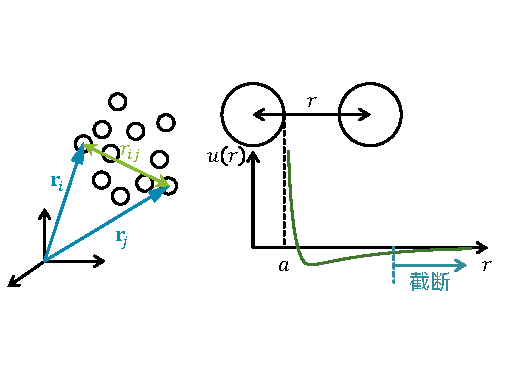
\includegraphics{../images/interaction_potential_energy.pdf}
  \caption{用于说明粒子相互作用势的示意图。任意两个粒子$i$和$j$的相互作用势依赖它们的距离$r_{ij}$,可由热能函数$u\left(r\right)$来描述。对于硬球粒子,$r$的取值范围是$\left[2a,\infty\right)$,$a$是粒子的半径。无论$u\left(r\right)$的具体形式,在$r\rightarrow \infty$时$u$总是趋于零。因此为了简化可设置某截断值,不考虑距离大于这个值的粒子间作用势(见正文介绍)。}
  \label{fig:interaction_potential_energy}
\end{figure}

式\eqref{eq:III.1_potential_energy_sum_two_body}的双重求和,需要我们在每一瞬间的定格下,把每对粒子的位置所对应的$r_{ij}$代入$u\left(r_{ij}\right)$算出势能值,再把它们全加起来。这个行务的艰巨性是天文级的。为了简化,我们讨论一下相互作用势的距离截断。惯例上,相互作用势能$u\left(r\right)$一般规定在$r\rightarrow\infty$处绝对单调地趋于零,于是我们可以认为距离大于某个值的两个粒子的势能贡献小到可以忽略,从而少算很多对粒子。这就是所谓的相互作用势的距离截断。以下以两个典型的相互作用势为例进行考察。

两个相同半径$a$的球形粒子间的范德华作用势是
\[u_\text{vdW}\left(r\right)=-\frac{A_\text{H}a}{6r}\]
其中$A_\text{H}$是Hamaker常数,它与粒子作为一个实际物质被诱导出偶极矩的难易程度有关,负号使作用势取负值,这是因为惯例上以负值的作用势表示吸引作用势。$A_\text{H}$的值一般在\qty{-e19}{\joule}到\qty{-e20}{\joule}。我们可以用热运动单位能量$k_\text{B}T$作为一个判据,如果吸引势能的大小小于$k_\text{B}T$,它将无法束缚粒子的热运动。由$\left|u_\text{vdW}\left(r\right)\right|<k_\text{B}T$得$r>A_\text{H}a/\left(6k_\text{B}T\right)\equiv r_\text{cut}$,$r_\text{cut}$是我们按这个标准定义的截断距离。在\qty{30}{\degreeCelsius}时,水分子($A_\text{H}=\qty{3.7e-20}{\joule}$)之间的作用势截断距离$r_\text{cut}\approx 1.5a$。可见,范德华势对总势能的贡献,一般只需考虑最相邻两粒子(nearest neighborhood)间的加和即可。

在水中,同种电荷的单价电解质之间的静电势
\[u_\text{el}\left(r\right)=\frac{1}{k_\text{B}T}\lambda_\text{B}\left(\frac{e^{\kappa a}}{1+\kappa a}\right)^2\frac{e^{-\kappa r}}{r}\]
其中$\lambda_\text{B}$是Bjerrum长度,$\kappa^{-1}$是Debye--Hückel屏蔽长度。在室温下,\qty{1}{\milli\mole\per\liter}的\ce{NaCl}水溶液,$\lambda_\text{B}\approx\qty{0.71}{\nano\meter},\kappa^{-1}\approx\qty{0.074}{\nano\meter}$。令$\left|u_\text{el}\left(r\right)\right|<k_\text{B}T$得$r_\text{cut}\approx \num{7.1}a$。可见,静电相互作用在两、三个分子的距离范围内都是十分重要的势能贡献。所以我们常说,范德华作用是短程作用,静电作用是长程作用。

尽管采用了截断距离的近似能让我们少算好多对粒子的势能,但这只对计算机模拟时减少计算量有利。在一定温度下,宏观上处于平衡态的系统,微观下粒子一直在运动。宏观性质的系统平均是按各微观状态出现概率求得的数学期望。如果只有草稿纸和铅笔,沿着上述思路是很难继续下去的。下面引入格子模型来进一步简化溶液的总内能的计算。

\subsection{格子模型}
我们假想溶液系统所占体积被划分成网格,格子的大小都相同。无论是溶剂还是溶质分子,每个分子只能放在一格中,这相当于认为溶质和溶剂分子的大小相同,且混合前后系统的体积不变,即$\Delta_\text{mix}V=0$。这件事最直接的效果是$\Delta_\text{mix}H=\Delta_\text{mix}U+p\Delta_\text{mix}V=\Delta_\text{mix}U$,因此讨论内能变化就相当于讨论了焓变。

\begin{wrapfigure}{r}{0.333\textwidth}
  \centering
  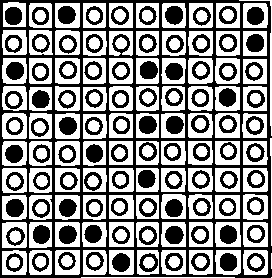
\includegraphics[width=\linewidth]{../images/lattice_binary_mixture.pdf}
  \caption{二元液体混合物中溶质分子在正规溶液格子模型中的分布示意图}
  \label{fig:lattice_binary_mixture}
\end{wrapfigure}

在3维空间中,我们可以设定这套网格的\emph{配位数(coordinate number)}$z$,即每个格子周围相邻的格子个数。在连续的三维空间中,尺寸相同的球的堆积密度与堆积的方式有关,造成不同的等效配位数。显然,需要$z\geq 2$才有可能构成可在三维空间中延展的网格结构。三维空间中大小相同的硬球的最紧密的堆砌方法是\emph{面心立方(face-centered cubic,FCC)}或\emph{六方密排(hexagonal close-packed,HCP)},它们的配位数都是\num{12}。因此$z$的理论上的取值范围须是\num{2}到\num{12},实际系统$z$一般大于\num{6}。此外,液体中的分子不是静止不动的;在任一瞬间,各分子都并不精确地落在一套周期性的晶格内。格子模型的配位数仅反映液态系统中平均而言每个分子邻近的分子数,故$z$可取\num{6}至\emph{12}间的任意一个有理数。

我们马上会看到,格子模型简化了我们考虑系统的总势能的难度。现在我们只考虑处于相邻格子的两个分子间的势能对总势能的贡献,这相当于取$r_\text{cut}=2a$。这对于仅有范德华作用势的系统是比较合理的近似。既然任意两个相邻分子的间距都是$2a$,那么溶液的分子间的势能只需考虑三个定值:
\[\varepsilon_{11}=u_{11}\left(2a\right),\quad\varepsilon_{22}=u_{12}\left(2a\right),\quad\varepsilon_{12}=u_{12}\left(2a\right)\]
其中$u_{11}\left(r\right)$、$u_{22}\left(r\right)$和$u_{12}\left(r\right)$分别是两溶剂分子间、两溶质分子间以及一溶剂分子与一溶质分子间的相互作用势能函数。由于分子种类不同,它们应是不同的势能函数。

之前已经说过,恒温过程内能变化仅依赖系统的平均势能的变化;只考虑二体相互作用势时,系统的总势能是各对粒子间作用势能之和。现在如果进一步只考虑最邻近两原子间的作用势能,那么系统的内能就是所有相邻格子间势能之和。为此我们规定一些记号和变量。如果记“($i$-$j$)”为组份$i$粒子和组份$j$粒子处于相邻格子的情况,$i,j=1,2$, 记$z P_{ij}$是网格中所有($i$-$j$)的个数\footnote{$P_{ij}$是一个概率,表示在任意两个相邻格子中,一个格子是组份$i$的粒子,另一个格子是组份$j$的粒子的概率。然而读者在这里只需要理解整个乘积$z P_{ij}$是($i$-$j$)的个数即可。},那么有
\[U_\text{溶液}=zP_{11}\varepsilon_{11}+zP_{12}\varepsilon_{12}+zP_{22}\varepsilon_{22}\]
我们可以通过以下讨论进一步把上式中的$P_{11}$和$P_{22}$用$P_{12}$表示。已知网格中放了$N_1$个溶剂分子,每个溶剂分子周围有$z$个格子,那么$N_1 z$这个数就把所有(1-1)相邻对计算了两次,再加上所有的(1-2)相邻对,写成式子就是
\[N_1z=2zP_{11}+zP_{12}\]
即
\[N_1=2P_{11}+P_{12}\]
同理有
\[N_2=2P_{22}+P_{12}\]
用这两个关系就可以消去$U_\text{溶液}$中的$P_{11}$和$P_{22}$,得
\[
  U_\text{溶液}=\frac{1}{2}N_1z\varepsilon_{11}+\frac{1}{2}N_2z\varepsilon_{22}+zP_{12}\Delta\varepsilon
\]
其中$\Delta\varepsilon=\varepsilon_{12}-\frac{1}{2}\left(\varepsilon_{11}+\varepsilon_{22}\right)$是\emph{交换能(interchange energy)}。

纯溶剂的内能,对应于上式$N_2=0$和$zP_{12}=0$的情况,纯溶质的类似,因此混合内能变就是
\begin{equation}\label{eq:III.1_mixing_internal_energy_regular_solution}
  \Delta_\text{mix}H=\Delta_\text{mix}U=zP_{12}\Delta\varepsilon
\end{equation}
记得由于我们假定了$\Delta_\text{mix} V=0$, 因此$\Delta_\text{mix}H=\Delta_\text{mix}U$,也体现在上式了。我们可以看到,在格子模型的帮助下,对于仅考虑最邻近两原子间的作用势能的系统,混合内能变的表达式写成了系统的化学特异性参数——$z$和$\Delta\varepsilon$——与混合物的组成参数$P_{12}$的乘积。诚然,$P_{12}$与溶液的组成$x_1$和$x_2$的直接关系,还有待推导,这将会在后面解决。

\subsection{溶液的熵的微观根源}
当分子数$N$非常大时,热力学系统在定温定压下或定温定容下某宏观状态的熵都近似于内能相同的孤立系统表达式,即
\[S\approx k_\text{B}\ln\Omega\]
其中$\Omega$是具有与实际关注的系统相同的分子数、相同的体积以及相同的内能的孤立系统的可取微观状态数。对于一个由$N$个微观粒子组成的经典力学系统,一组位置$\left(\mathbf{r}_1,\cdots,\mathbf{r}_N\right)$和动量$\left(\mathbf{p}_1,\cdots,\mathbf{p}_N\right)$的取值就唯一确定系统的一个微观状态。所以$\Omega$就是表示这个孤立系统在定温定容定内能下可以取多少种不同值的一组$\left(\mathbf{r}_1,\cdots,\mathbf{r}_N,\mathbf{p}_1,\cdots,\mathbf{p}_N\right)$。在连续空间的考虑方式下,这将是一个天文数字,但我们坚持继续讨论下去。

注意到,经典力系的动量与位置取值相互独立,意思是说,系统可以取的动量值个数不依赖系统已取的位置值,反之亦然。那么,若系统可取$\Omega_\text{m}$种动量值和$\Omega_c$种位置值\footnote{m代表动量(momentum);c代表位形(configuration)。},则总共可取的微观状态数将直接是它们的乘积$\Omega=\Omega_\text{m}\Omega_\text{c}$。再考虑到,溶质与溶剂混合前、后温度是相同的,由温度“平均动能”的物理意义,我们不难接受“混合前、后$\Omega_\text{m}$相同”的说法\footnote{严格的统计力学理由待补充。}。此时混合前后系统的熵变化
\[\begin{aligned}\Delta_\text{mix}S & =S_\text{溶液}-S_\text{纯组份}                                                                                  \\
                                  & =k_\text{B}\left(\ln\Omega_\text{m}+\ln\Omega_\text{c,溶液}-\ln\Omega_\text{m}-\ln\Omega_\text{c,纯组份}\right) \\
                                  & =k_\text{B}\left(\ln\Omega_\text{c,溶液}-\ln\Omega_\text{c,纯组份}\right)                                       \\
                                  & =\Delta_\text{mix}S_\text{c}\end{aligned}\]
其中$S_\text{c}=k_\text{B}\ln\Omega_\text{c}$叫\emph{位形熵(configurational entropy)}。上式表明,对于等温混合过程,只需统计混合前后位形数$\Omega_\text{c}$——即分子空间排布的方法数——的变化,就能得到系统的混合熵变了。

在格子模型中,分子空间排布的方法数可抽象成一个组合数问题。若考虑把$N_1$个溶剂分子和$N_2$个溶质分子\emph{依次}放入$N=N_1+N_2$个格子中,总共有$N!$种放法。但由于同组分的分子是不可区分的,因此还要除以$N_1!N_2!$。于是溶液的位形数是
\begin{equation}
  \Omega_\text{c,溶液}=\frac{N!}{N_1!N_2!}
  \label{eq:III.1_omega_c_solution}
\end{equation}
在混合前,组份1和2处于纯物质状态,相当于把$N_1$个溶剂分子放入一个盒子中,以及把$N_2$个溶剂分子放入第二个盒子中的方法——只有一种。因此$\Omega_\text{c,纯组份}=1$,$S_\text{c,纯组份}=0$。混合熵变就是
\[\begin{aligned}
    \Delta_\text{mix}S & =k_\text{B}\ln\Omega_\text{c,溶液}                                                     \\
                       & =k_\text{B}\left[\ln\left(N!\right)-\ln\left(N_1!\right)-\ln\left(N_2!\right)\right]
  \end{aligned}\]
当$N$很大时,可以用\emph{Stirling近似(Stirling's approximation)}:
\[\ln\left(N!\right)\approx N\ln N-N\]
代入上式,得
\begin{equation}\label{eq:III.1_mixing_entropy_regular_solution}
  \Delta_\text{mix}S=-k_\text{B}\left(N_1\ln x_1+N_2\ln x_2\right)
\end{equation}
我们发现,这个混合熵变表达式恰好是理想溶液的混合熵变表达式(式\eqref{eq:II.4_ideal_mixture_mixing_function_nonzero}的双组份情况)。

把构形熵直接估计为上述的组合问题,暗中假定了,每个格子放什么球,不受周围格子放置方式的限制。实际情况中,如果不同的构形的总势能不同,那么在恒温条件下,不同构形出现的概率是不均等的,而应该按照构形的总势能来加权平均。这件事情将会在下一节仔细讨论。现在既然得到了理想混合物的混合熵变表达式,那说明理想溶液可理解为不同分子构形势能差别可忽略的一种理想情况。按照上一小节关于混合内能变的讨论,则就算仅考虑最相邻对作用势,也仍需$\Delta\varepsilon=0$,那就是彻底要求$\Delta_\text{mix}U=\Delta_\text{mix}H=0$——这也正是理想溶液的热力学条件。我们知道,理想混合物的混合熵变是由理想溶液的热力学定义和基本热力学关系所规定的。这里我们通过格子模型的微观模型的推导复现出了理想溶液的混合熵变表达式。我们因此可以认为,尽管格子模型作了各种简化假定,但它基本抓住了溶液的微观机理。
\end{document}